\documentclass[10pt,twocolumn,letterpaper]{article}

\usepackage{cvpr}
\usepackage{times}
\usepackage{epsfig}
\usepackage{graphicx}
\usepackage{amsmath}
\usepackage{amssymb}
\usepackage{svg}
\usepackage{currfile}
\usepackage{minibox}
\usepackage{longtable}
\usepackage{bm}

\usepackage[breaklinks=true,bookmarks=false]{hyperref}

\cvprfinalcopy

\def\cvprPaperId{****}
\def\httilde{\mbox{\tt\raisebox{-.5ex}{\symbol{126}}}}

\setcounter{page}{1}
\begin{document}

\title{ Exploiting synthetic images for real-world image recognition }

\author{Max Maton\\
Delft University of Technology\\
Delft, The Netherlands\\
{\tt\small https://in.maxmaton.nl/}
\and
Jan van Gemert\\
Delft University of Technology\\
Delft, The Netherlands\\
{\tt\small http://jvgemert.github.io/}
\and
Miriam Huijser\\
Aiir Innovations\\
Amsterdam, The Netherlands\\
{\tt\small https://aiir.nl/}
\and
Osman Kayhan\\
Delft University of Technology\\
Delft, The Netherlands\\
{\tt\small o.s.kayhan@tudelft.nl}
}

\maketitle

\iffalse
Abstract
</h2>
<p>
\fi

\begin{abstract}
Creating big datasets is often difficult or expensive which causes people to try to augment their dataset with rendered images. This often fails to significantly improve accuracy due to a difference in distribution between real and rendered datasets.
This paper shows that the gap between synthetic and real-world image distributions can be closed by using a GAN to convert the synthetic data to a dataset which has the same distribution as the real data. Training this GAN requires only a fraction of the dataset traditionally required to get a high classification accuracy. This converted data can subsequently be used to train a classifier with a higher accuracy than a classifier trained only on the real dataset.

\end{abstract}

\begin{figure}[h]
\begin{center}
{\scriptsize \includesvg[width=0.85\linewidth]{../method.svg}}
\end{center}
   \caption{Technique used to convert the rendered dataset for use in training.}
\label{fig:method}
\end{figure}

\section{Introduction}

Deep learning has revolutionised visual object recognition. Thanks to huge datasets and fast hardware (GPUs), current object recognition approaches have near-human accuracy.
%<p>
Because creating big datasets is often very expensive, people start to turn to rendered images to augment their datasets. However, training networks on rendered images may not achieve the desired accuracy due to a gap between synthetic and real image distributions \cite{10.1.1.151.7688}.
%<p>
Another development in current research is the increased focus on Generative Adversarial Networks (GANs) to generate images that look similar to the images they were trained on \cite{1406.2661}.
%<p>
In this paper the impact of the distribution gap between synthetic and real image distributions is decreased by using a GAN to modify rendered images to have the same distribution as real images. This technique is shown to be useful for inflating very small datasets to a level where they can be used to more create accurate classifiers.

\section{Related work}
Rendered data can sometimes be used to train networks, i.e. facial expression analysis using rendered faces \cite{Abbasnejad_2017_ICCV}, using rendered images to segment images of indoor scenes \cite{10.1.1.94.777} and font character classification trained on interpolated real samples \cite{10.1.1.151.7688}. These networks are trained by creating a rendered dataset that is as close as possible in statistical distribution as the real dataset. Generally this is very difficult or expensive to achieve.

%<p>
The problem of creating rendered datasets with a distribution close to a real dataset can be solved by using domain adaptation. This is generally done using Generative Adversarial Networks \cite{10.1109/CVPR.2017.18, 10.1007/978-3-319-58347-1, 1703.05192.pdf} trained to create samples based on images in the rendered dataset that are indistinguisable from images in the real dataset. We decided to perform this research on the GAN as described by Bousmalis et al\footnote{We chose to base our research on this paper due to the available TensorFlow\cite{tensorflow} implementation} \cite{10.1109/CVPR.2017.18}.


\section{Inflating datasets using rendered data and GANs}

\begin{figure}[h]
\begin{center}
{\scriptsize \includesvg[width=0.85\linewidth]{../GAN.svg}}
\end{center}
   \caption{Overview of the GAN architecture.}
\label{fig:gan-architecture}
\end{figure}

The basis of this research is a GAN that converts images from a rendered dataset distribution to an image that appears to come from the distribution of a real dataset. This GAN consists of three parts which are shown in figure \ref{fig:gan-architecture}. The first part is a generator network that does the image conversion. The second part of the GAN is a discriminator, which tries to distinguish between the output of the generator and images from the real dataset. The third part of the GAN is a classifier that predicts the label of images coming from either the real dataset, the generator or the rendered dataset. All these networks are trained in parallel. The discriminator and classifier are trained to reduce the amount of misclassifications. The generator is trained to minimise the amount of pixels changed in the image, to minimise the loss in classification by the classifier and to try to fool the discriminator to classify the image as real.

%<p>
To test the effects of inflating datasets when using this technique, we first trained the GAN with a real and rendered dataset. We then apply the trained GAN on the rendered dataset to create a new synthetic dataset. A combined dataset consisting of the synthetic dataset and the real dataset was used to train a second classifier.

\section{Experiments}


We evaluated this technique on the MNIST dataset \cite{mnist} together with a rendered dataset generated by rendering open source font digits in multiple rotations for all number classes.
%<p>
The rendered dataset contains samples from $149$ fonts, with each digit rendered having $47$ variations each with a distinct rotation between $-47$ and $46$ degrees. All images were normalised using the same algorithm used to normalise the MNIST samples, the result of which can be seen in figure \ref{fig:example-font-images}. A random sample of $10,030$ of those images were put in a test set and the remaining $60,000$ images were used as the rendered dataset.

\begin{figure}[t]
\begin{center}
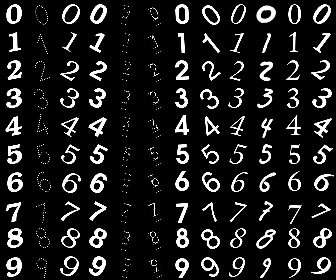
\includegraphics[width=0.7\linewidth]{example-font-images.png}%
\end{center}
   \caption{Example images of the MNIST font dataset.}
\label{fig:example-font-images}
\end{figure}

%<p>
The GAN was modified to use $10\%$ of the training data as a validation set instead of a constant $1,000$ samples as this allowed for smaller sample sizes.

%<p>
For multiple ratios\footnote{ Ratios used were: $0.001$, $0.003$, $0.005$, $0.007$, $0.008$, $0.024$, $0.056$, $0.1$, $0.3$, $0.5$, $0.7$ and $0.9$. } r, where $0 > r > 1$, we created the following datasets:

\begin{description}
	\item{$\text{MNIST}_\text{original}$} \hfill \\ $60,000 \times r$ images from the original MNIST dataset.
	\item{$\text{MNIST}_\text{font}$} \hfill \\ $60,000 \times (1 - r)$ images from the rendered font dataset.
\end{description}

%<p>
We used these two datasets to train the GAN using $375,000$ steps with batchsize $32$ and subsequently applied the trained GAN on the $\text{MNIST}_\text{font}$ dataset to create the $\text{MNIST}_\text{GAN}$ dataset. This made the $\text{MNIST}_\text{GAN}$ dataset have the exact same size as $\text{MNIST}_\text{font}$.

%<p>
\clearpage
With these datasets we trained five instances of the following classifiers:

\begin{description}
	\item{$5\times \text{C-MNIST}_\text{original}$} \hfill \\ Classifier only trained on $\text{MNIST}_\text{original}$
	\item{$5\times \text{C-MNIST}_\text{font}$} \hfill \\ Classifier only trained on $\text{MNIST}_\text{font}$
	\item{$5\times \text{C-MNIST}_\text{GAN}$} \hfill \\ Classifier only trained on $\text{MNIST}_\text{GAN}$
	\item{$5\times \text{C-MNIST}_\text{original+GAN}$} \hfill \\ Classifier only trained on $\text{MNIST}_\text{original+GAN}$
	\item{$5\times \text{C-MNIST}_\text{original+font}$} \hfill \\ Classifier only trained on $\text{MNIST}_\text{original+font}$
\end{description}

%<p>
Each classifier was tested on the MNIST test set which resulted in an classification accuracy.

\section{Results}

%<p>
To validate whether the GAN was creating useful images, we looked at the resulting images in $\text{MNIST}_\text{GAN}$ examples of which can be seen in Figure \ref{fig:results}.

\begin{figure}[h]
\begin{center}
	\parbox{0.7\linewidth}{ \center \small $r = 0.001$ 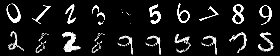
\includegraphics[width=0.8\linewidth]{results-001.png} }
	\parbox{0.7\linewidth}{ \center \small $r = 0.007$ 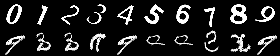
\includegraphics[width=0.8\linewidth]{results-007.png} }
	\parbox{0.7\linewidth}{ \center \small $r = 0.100$ 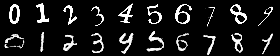
\includegraphics[width=0.8\linewidth]{results-100.png} }
	\parbox{0.7\linewidth}{ \center \small $r = 0.700$ 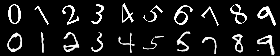
\includegraphics[width=0.8\linewidth]{results-700.png} }
\end{center}
   \caption{Example images of the MNIST font dataset. Top of each image is from $\text{MNIST}_\text{font}$, bottom is the generated image in $\text{MNIST}_\text{GAN}$. }
\label{fig:results}
\end{figure}

%<p>
From visual inspection it is apparent that the GAN has trouble keeping the labels consistent if there is not enough real training data. An example of this are the 1 and the 2 of $r = 0.007$ in figure \ref{fig:results}: they both result in something that looks like the same 8 instead of something that looks like a 1 or 2 respectively. This means that the classifier trained on this new dataset will receive two very similar samples with conflicting labels. We measured the accuracy on MNIST of $\text{C-MNIST}_\text{GAN}$ and found low accuracy for lower ratios. This supports the conclusion that there is an issue with labeling when the GAN is not trained with enough real data.

\subsection{\boldmath\bfseries $\text{C-MNIST}_\text{font}$ performance}
\begin{figure}[h]
\begin{center}
	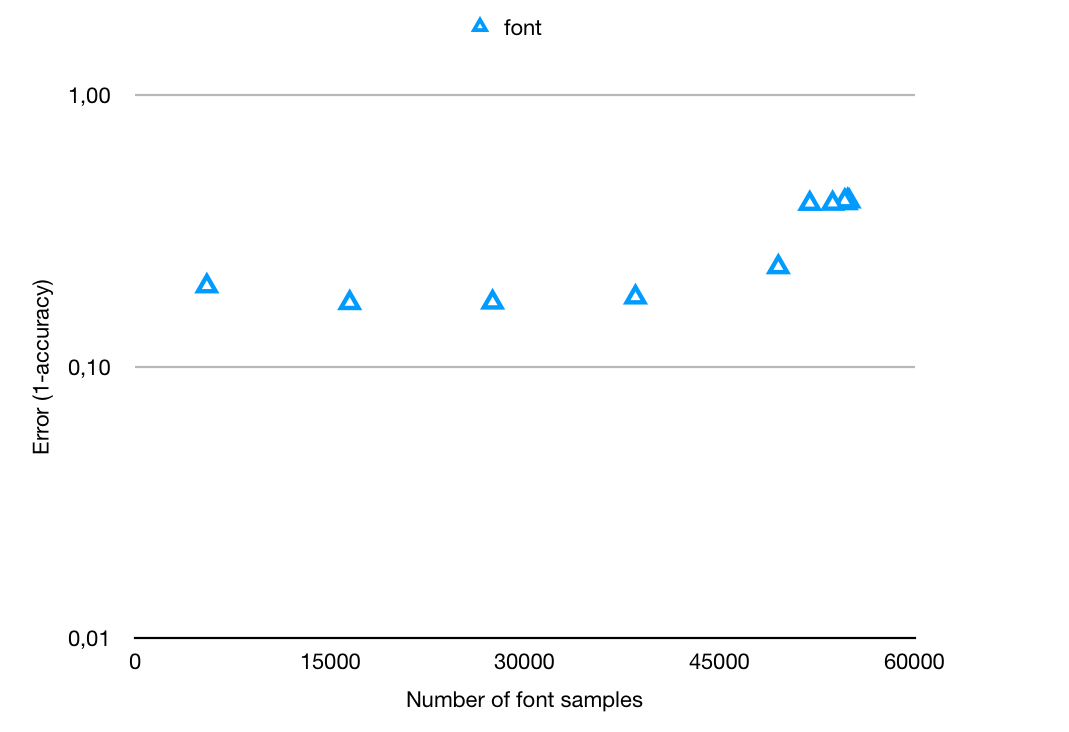
\includegraphics[width=0.9\linewidth]{../graph-font.png}
\end{center}
   \caption{Performance of $\text{C-MNIST}_\text{font}$ with varying amounts of $\text{MNIST}_\text{font}$ training data. Performance decreases with more training samples indicating that $\text{MNIST}_\text{original}$ and $\text{MNIST}_\text{font}$ have different characteristics.}
\label{fig:graph-font}
\end{figure}

To make sure we actually test whether the GAN is able to close the distribution gap we looked at the accuracy of $\text{C-MNIST}_\text{font}$. For this dataset the error shows an inverse relation between the amount of samples and the performance of the classifier, which can be seen in figure \ref{fig:graph-font}. This indicates that a gap exists between the rendered font dataset and the MNIST test dataset.


\subsection{\boldmath\bfseries $\text{C-MNIST}_\text{original}$ versus $\text{C-MNIST}_\text{original+GAN}$}
\begin{figure}[h]
\begin{center}
	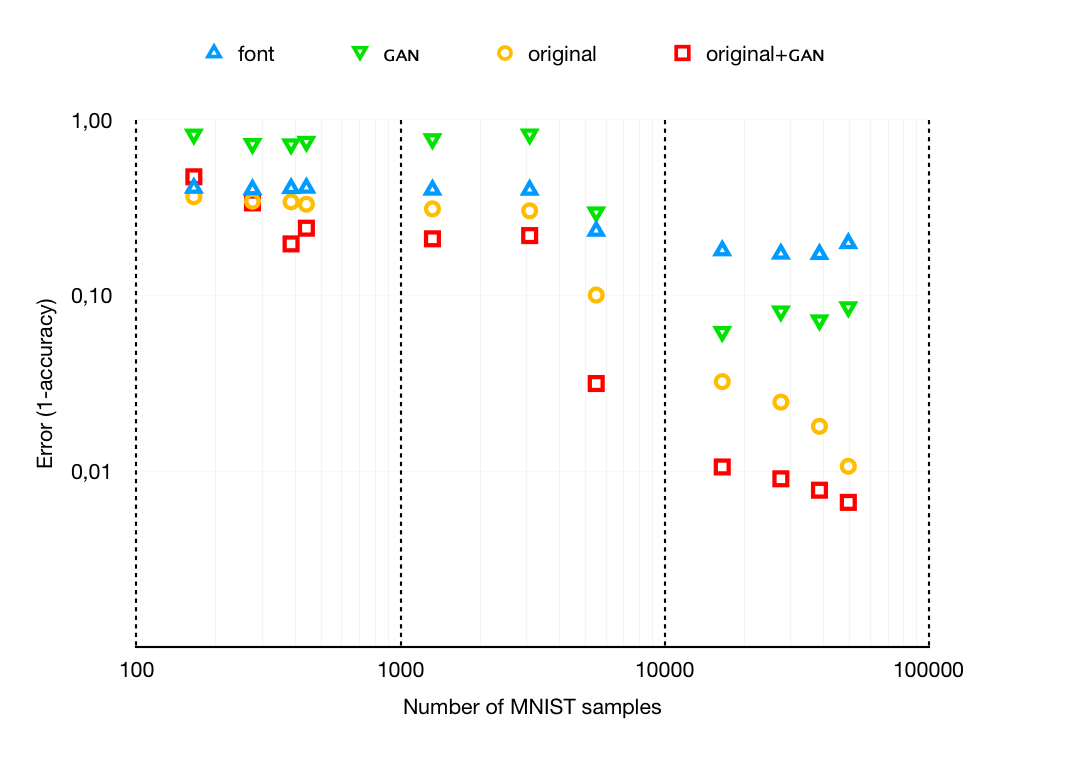
\includegraphics[width=0.9\linewidth]{../graph-results.png}
\end{center}
   \caption{Performance of classifiers with different amounts of MNIST training data. Training with the GAN data improves results after a minimal amount of original MNIST samples.}
\label{fig:graph-results}
\end{figure}


We compared the accuracy of $\text{C-MNIST}_\text{font}$, $\text{C-MNIST}_\text{GAN}$, $\text{C-MNIST}_\text{original}$ and $\text{C-MNIST}_\text{original+GAN}$ to see whether training with the $\text{MNIST}_\text{original+GAN}$ dataset is better than training with one of the individual datasets. The result of this comparison can be seen in figure \ref{fig:graph-results}.


$\text{C-MNIST}_\text{original+GAN}$ is only more accurate than the $\text{C-MNIST}_\text{original}$ when the GAN is trained on more than 385 real images ($r = 0.007$). There seems to be a minimum amount of real samples after which the GAN starts to produce meaningful data.

Using MNIST as a test case, this technique is able to close the distribution gap even with as little $0.7\%$ real data in the resulting dataset.

\begin{figure}[h]
\begin{center}
	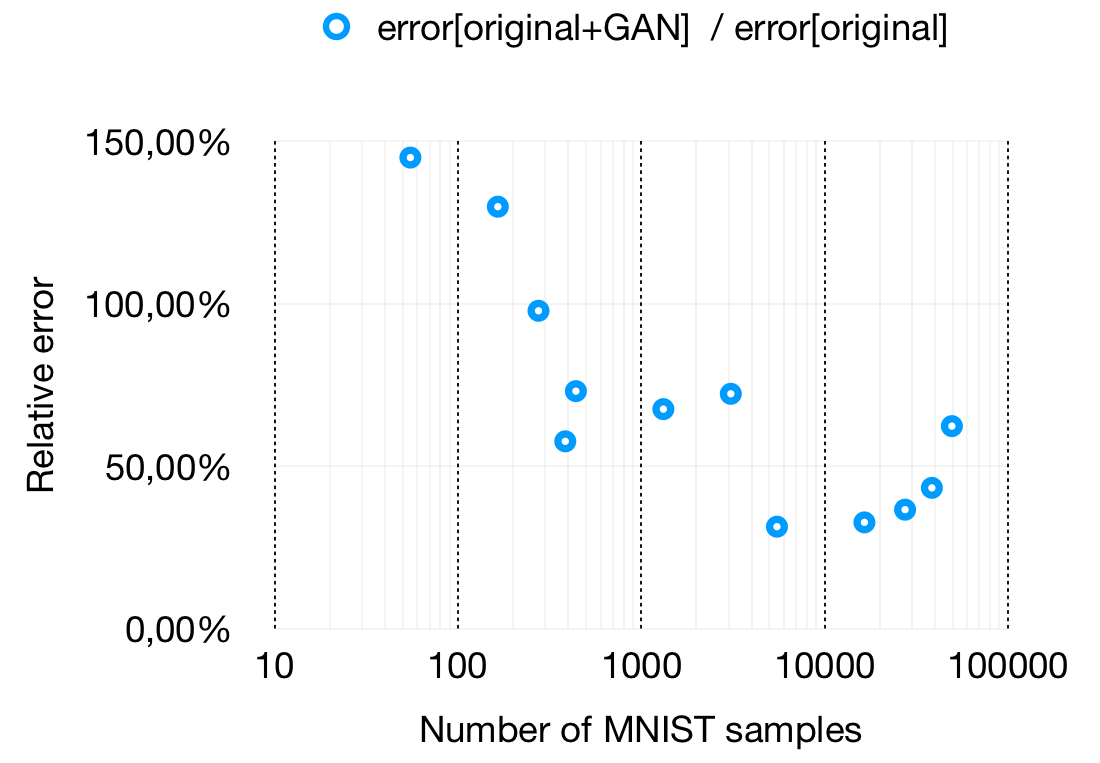
\includegraphics[width=0.9\linewidth]{../graph-error-comparison.png}
\end{center}
   \caption{Error of $\text{C-MNIST}_\text{original+GAN}$ compared to the error of $\text{C-MNIST}_\text{original}$, lower is better. Lowest relative error was found at $5,500$ MNIST samples.}
\label{fig:graph-relative-error}
\end{figure}

We also compared the difference in wrong predictions between $\text{C-MNIST}_\text{original}$ and $\text{C-MNIST}_\text{original+GAN}$. As is shown in figure \ref{fig:graph-relative-error}, the highest reduction in error was achieved with $5,500$ MNIST images and $49,500$ font images. This indicates that for MNIST, this technique becomes more effective when the ratio between real and rendered images becomes less extreme.

\subsection{\boldmath\bfseries $\text{C-MNIST}_\text{original}$ against $\text{C-MNIST}_\text{original+font}$}
\begin{figure}[h]
\begin{center}
	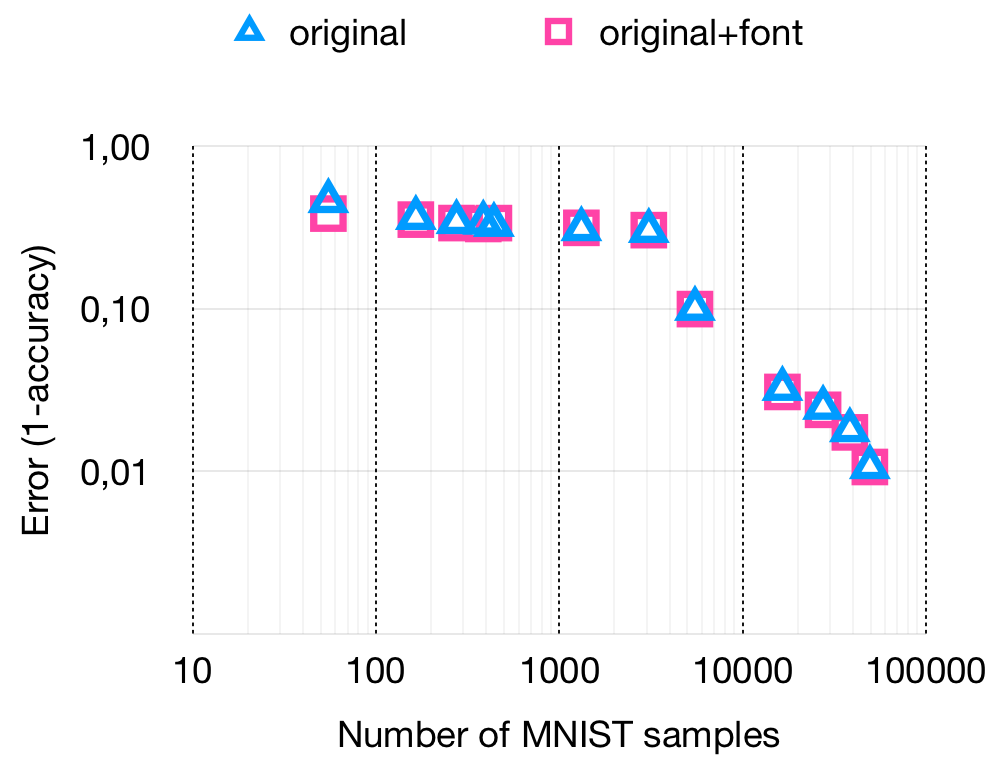
\includegraphics[width=0.9\linewidth]{../graph-font-original-comparison.png}
\end{center}
   \caption{Performance of $\text{C-MNIST}_\text{original+font}$ versus the performance of $\text{C-MNIST}_\text{original}$ for varying amounts of training data. Performance is almost the same indicating no advantage to including font data in the training set directly.}
\label{fig:graph-font-original-comparison}
\end{figure}

%<p>
To confirm that the improved results of $\text{C-MNIST}_\text{original+GAN}$ can not be solely explained by the addition of the rendered font data, we compared $\text{C-MNIST}_\text{original}$ with $\text{C-MNIST}_\text{original+font}$ to see if the addition of font data increased the accuracy. From the results in figure \ref{fig:graph-font-original-comparison} we had to conclude that $\text{C-MNIST}_\text{original+font}$ has performance roughly equal to $\text{C-MNIST}_\text{original}$ at the ratios where $\text{C-MNIST}_\text{original+GAN}$ is more accurate. The addition of more font data cannot explain the additional accuracy of $\text{C-MNIST}_\text{original+GAN}$ indicating this increase is a property of the transformation made by the GAN.


\section{Discussion}

Due to a limited amount of time, no finetuning has been done on the other hyperparameters of the GAN. Optimizing these hyperparameters might further improve classification accuracy which should result in a further reduction in the amount of required samples from the real dataset.

When measuring the performance of $\text{C-MNIST}_\text{original+GAN}$ versus $\text{C-MNIST}_\text{original}$ we found that even though the generated samples are not good samples for their target class, $\text{C-MNIST}_\text{original+GAN}$ quickly becomes much more accurate than $\text{C-MNIST}_\text{original}$ before the samples look like useful samples. This effect can partially be explained by results shown by Sukhbaatar et al. that indicate that deep learning is robust to massive label noise \cite{Sukhbaatar2014TrainingCN}. This would mean that the network is still capable of learning higher level features from the mislabeled samples and is able to succesfully ignore the bad labeling.


\section{Conclusion}
Our goal was to use a GAN to close the distribution gap between rendered and real datasets. 

Using MNIST as an example, we were able to show that it's possible to create a rendered dataset. We've shown that a distribution gap exists between the dataset we created and the real MNIST dataset and were able to close this gap using our described technique.

We've shown that GANs can be used to inflate trainingsets by reducing the gap between synthetic and real datasets. Furthermore, they can do so with very little real training data. This technique can be very useful for problems where only a small real dataset is available.

{\small
\bibliographystyle{ieee}
\bibliography{references}
}

\onecolumn
\appendix

\section{Raw experiment results}
\begin{longtable}{ | l | l | l | l | l | l | l | }
	\hline
	\input{results.tex}
\end{longtable}

\end{document}
